In order to deeply understand and reconstruct cellular mechanisms influenced by drug treatments, pathologies or diseases, it is fundamental to look at multiple omics data types at the same time.

Previous chapters deeply described tools for multiple omics data analysis, integration and visualization using command line tools.
Even if the command line approach is pretty common inside the bioinformatics community, it is not for every scientist who is not so confident with programming languages or terminal.
When working with multiple omics data, there is an overabundance of available tools for each sequencing that can bewilder a beginner, up to the point to renounce approaching the analysis problem.

%Moreover, thanks to our previous experiences \cite{russo2015advantages} in developing \gls{gui}, we noticed a growing interest by the scientific community in using interactive software.
%This interest seems to be leaded by multiple motivations, such as the need to analyze data very fast or the lack of time in learning programming languages and terminal-line based tools.

Furthermore, even if the bioinformatics community has massively moved on the development of novel statistical and computational methods for multi-omics data integration, part of the scientific community is still anchored to the single-omics analysis side.
Even if still really helpful, it is still very common to read published papers based on single-omics data analysis without taking into account possible integrated solution with other omics data types.

Of course, it is not so simple to afford for multiple omics data experiments, but, nowadays, the internet swarms of public datasets.
In particular when looking at public biological data banks, such as \gls{geo}\footnote{\url{https://www.ncbi.nlm.nih.gov/geo/}} \cite{Services2007} or \gls{tcga}\footnote{\url{https://cancergenome.nih.gov/}} \cite{tcga2013a}, where it is possible to retrieve as many data as needed.

On the other side, if there are not so many papers publishing integrated analysis, it is also difficult for analysts to retrieve the right methodologies for the multi-omics data analysis and their visualization. 

\begin{figure}[H]
\centering
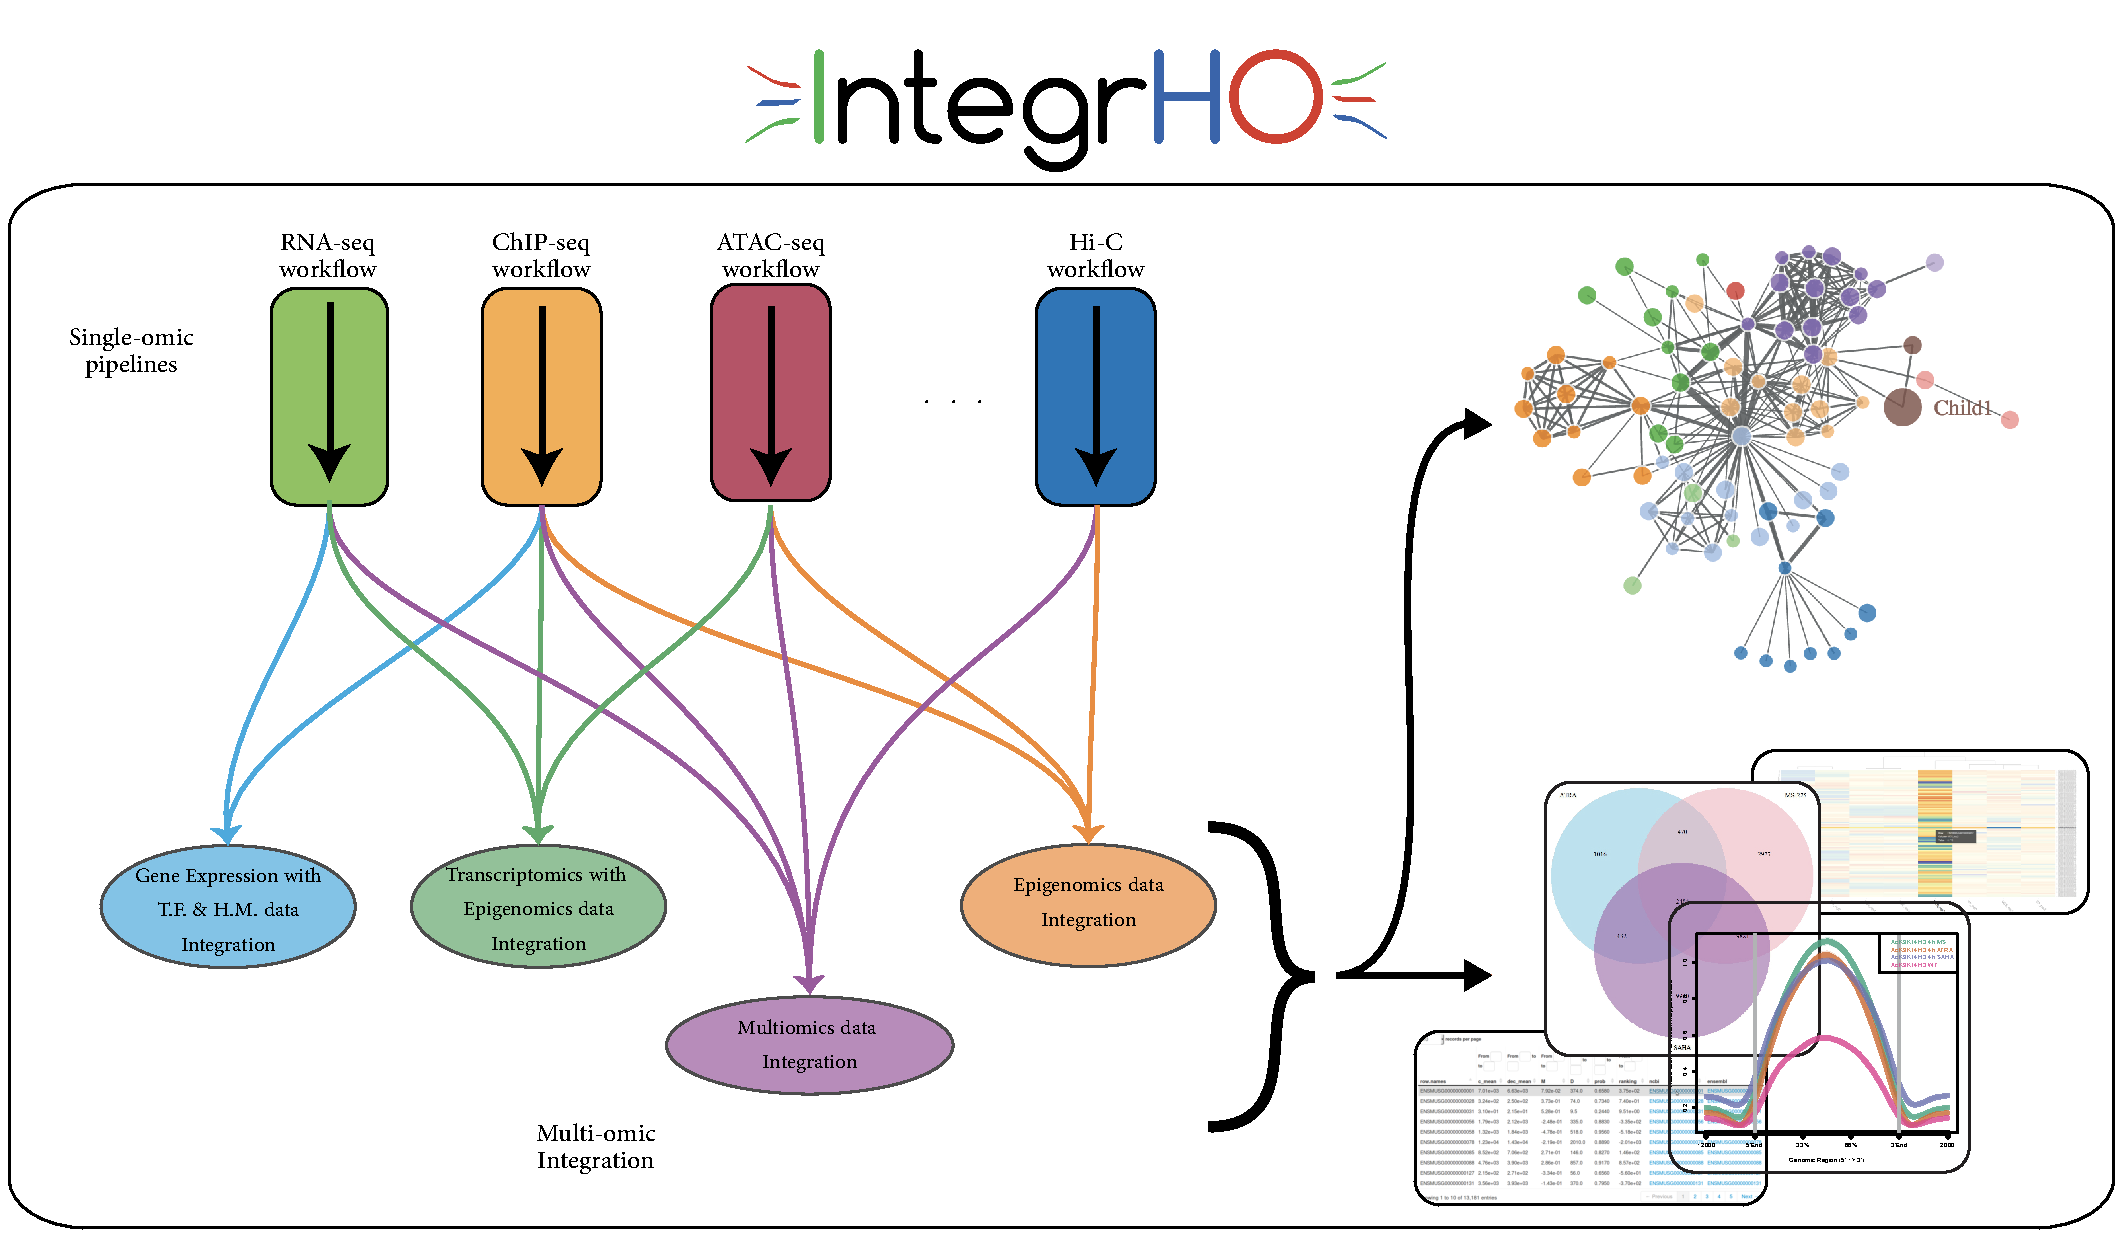
\includegraphics[width=\textwidth, keepaspectratio]{img/integrho/integrho_scheme.pdf}
\caption[\gls{igro} representation]{A schematical representation of \gls{igro} underlying idea.
Single-omics analysis methods are proposed in order to facilitate their multiple integration.
This integration can lead to produce graphical results, in case of low dimension datasets, or to more sophisticated integration model such as regulation networks, in case of high-dimension datasets.}
\label{fig:integrhoidea}
\end{figure}

Based on these considerations and in order to promote the multi-omics data integration, we decided to provide the scientific community of a novel easy-to-use instrument which not only gives the possibility to analyze single-omics data types but also guides the user through multiple ways of integrating multi-omics data types (figure \ref{fig:integrhoidea} gives an underlying idea of \gls{igro}).





%Several interface-based tools \cite{Poplawski2016} have been proposed during last years but too often they are oriented to analyze singular-omics or when designed for multi-omics, they are pipeline oriented. 

%In this chapter we introduce \gls{igro}, our web-based platform for multi-omics data analysis and integration,  in a \gls{rr} spirit.


